%%%%%%%%%%%%%%%%%%%%%%%%%%%%%%%%%%%%%%%%%%%%%%%%%%%%%%%%%%%%%%%%%%%%%%%%%%%%%%%%
%2345678901234567890123456789012345678901234567890123456789012345678901234567890
%        1         2         3         4         5         6         7         8

\documentclass[letterpaper, 10 pt, conference]{ieeeconf}  % Comment this line out if you need a4paper

%\documentclass[a4paper, 10pt, conference]{ieeeconf}      % Use this line for a4 paper

\IEEEoverridecommandlockouts                              % This command is only needed if you want to use the \thanks command

\overrideIEEEmargins                                      % Needed to meet printer requirements.

% See the \addtolength command later in the file to balance the column lengths
% on the last page of the document

% The following packages can be found on http:\\www.ctan.org
\usepackage{graphicx} % for pdf, bitmapped graphics files
\usepackage{subcaption}
%\usepackage{epsfig} % for postscript graphics files
%\usepackage{mathptmx} % assumes new font selection scheme installed
%\usepackage{times} % assumes new font selection scheme installed
%\usepackage{amsmath} % assumes amsmath package installed
%\usepackage{amssymb}  % assumes amsmath package installed

\title{\LARGE \bf
% Preparation of Papers for IEEE Sponsored Conferences \& Symposia*
Movie Rating Predictor Using Nonnegative Matrix Factorization on Tag Data
}


\author{Claire Chang, Thaxter Shaw, and TJ Tsai$^{1}$% <-this % stops a space
\thanks{$^{1}$T. Tsai is with the Department of Engineering at Harvey Mudd College,
301 Platt Blvd., Claremont, CA 91711. E-mail: {\tt\small ttsai@hmc.edu}}%
}



\begin{document}



\maketitle
\thispagestyle{empty}
\pagestyle{empty}


%%%%%%%%%%%%%%%%%%%%%%%%%%%%%%%%%%%%%%%%%%%%%%%%%%%%%%%%%%%%%%%%%%%%%%%%%%%%%%%%
\begin{abstract}

The goal of recommendation systems is to suggest suitable content such as movies, groceries, and more. This article aims to predict what someone will rate a movie, which could in turn be applied to a movie recommendation system. We propose a method of addressing this problem 

\end{abstract}


%%%%%%%%%%%%%%%%%%%%%%%%%%%%%%%%%%%%%%%%%%%%%%%%%%%%%%%%%%%%%%%%%%%%%%%%%%%%%%%%
\section{INTRODUCTION}

The goal of this paper is to predict what someone will rate a movie on a five-star scale.
This prediction can be used in recommendation systems for not only movies, but also grocery shopping, music, and more \cite{recsys}.

There are several obstacles that make this problem challenging. 
One issue, as investigated by Bell et al. is the effect of time. Over time, users may change their baseline rating (for example, have higher expectations of graphics) and begin to prefer different genres and actors \cite{netflix}.
Movies themselves also become more or less popular over time \cite{netflix}.

One approach that has been taken is to use a "neighborhood approach" that compares different movies, and recommends a highly rated movie that is similar to other movies a user has liked. 
Another approach is to use collaborative filtering (CF) methods such as nonnegative matrix factorization (NMF) and singular value decomposition (SVD) \cite{cf}. 
We could also use a hybrid approach of the neighborhood and CF approahces \cite{hybrid}.

In this paper, we use data from MovieLens. The dataset we use contains ratings of over 1000 movies made by various users, filtered such that each user has rated at least 20 movies.
The dataset also relates each movie to a series of short tags, such as "sci-fi," "cliché," or "overrated." This data was collected through users applying labels to movies, and machine learning \cite{lenskit}.


Our system uses NMF on this tag data to create clusters of tags, which we will equate to "genres". We then use these genres predict ratings. Finally, we use mean movie ratings to adjust this predicted rating.


\section{SYSTEM DESCRIPTION}

\begin{figure}[h]
   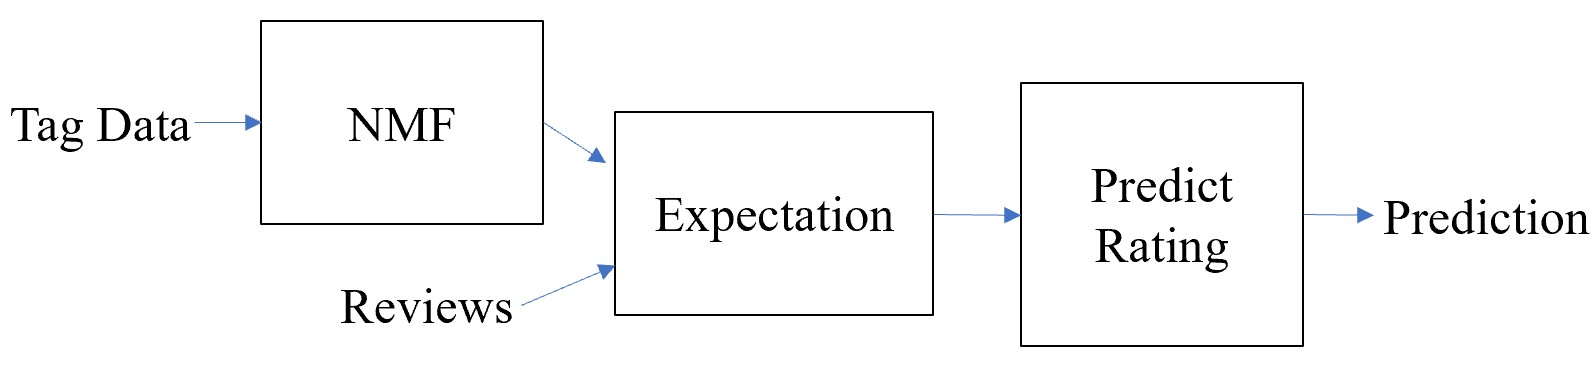
\includegraphics[scale=0.5]{./figs/blockdiagram.jpg}
   \caption{Block diagram of proposed system.}
\end{figure}

The overall architecture for our system is shown in Figure 1.

\subsection{Nonnegative Matrix Factorization}

We begin with the tag data, stored as a matrix of $t$ rows and $m$ columns. Here, $t$ is the number of tags and $m$ is the number of movies in the dataset.
We perform NMF on the tag data matrix, which gives us a template matrix $W$ and an activation matrix $H$.
In W, we have $t$ rows and $R$ columns, where $R$ represents the number of templates. In $H$, we have $R$ rows and $m$ columns.

Each template is comprised of clusters of tags and represents a genre. For example, the romantic comedy genre might contain the tags "cliché," "romance," "Ryan Gosling," and "comedy." In $H$, each movie is broken down into its component genres.

\subsection{Expectation}

Next, we assemble a new matrix of reviews. This matrix has $m$ rows and $p$ columns, where $p$ is the number of reviewers, and stores all ratings made by each user.

Then, we create another matrix $M$, which represents each reviewer's affinity to each genre. 
$M$ has $R$ rows and $p$ columns. Each entry in $M$ is an rating out of five stars indicating what a reviewer is expected to rate a typical movie from a given genre.
We get this information by taking the "expectation" of all the reviewer's ratings. In this expectation, ratings of movies more relevant to the genre of interest (as defined in $H$) are given more weight.

\subsection{Predict Rating}
Finally, we generate a predicted rating for a movie and reviewer from a query. For example, suppose we want to predict what reviewer A will rate the movie \textit{La La Land}. To do this, we will use a "genre fingerprint" for our movie.

Recall that $H$ is an $R \times m$ matrix, representing the relevance of each genre to each movie. We can $L1$ normalize the columns of $H$ to create a matrix storing the genre fingerprints of each movie.
These fingerprints indicate the breakdown of the movie into its component genres, such that each genre represents a proportion of the entire movie. See Figure 2 for examples of genre fingerprints.

For our example, let's assume that \textit{La La Land}'s fingerprint is 75\% romantic comedy and 25\% drama. Then, based on reviewer A's preferences for these genres (from matrix $M$), we can generate a preliminary prediction for their rating.

Finally, we look at the mean movie rating for \textit{La La Land}. If this mean rating is higher than our preliminary prediction, we round up to the nearest half-star. Otherwise, we round down.

\begin{figure*}[h]
   \begin{subfigure}[b]{\columnwidth}
      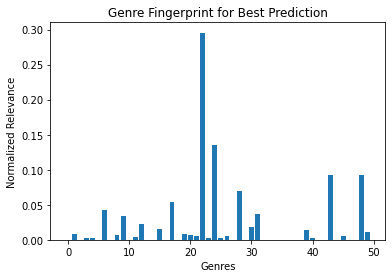
\includegraphics[width=\linewidth]{./figs/bestfingerprint.png}
      \caption{Fingerprint of movie from good prediction.}
   \end{subfigure}
   \hfill
   \begin{subfigure}[b]{\columnwidth}
      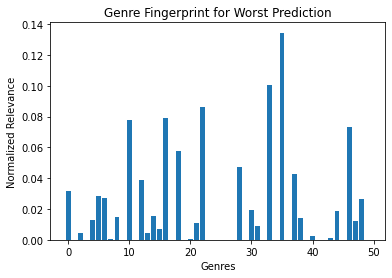
\includegraphics[width=\linewidth]{./figs/worstfingerprint.png}
      \caption{Fingerprint of movie from bad prediction.}
   \end{subfigure}
   \caption{Fingerprints of two movies. A fingerprint is the breakdown of the movie into genres. We can see that the fingerprint of the movie from the bad prediction has a wider distribution.}
\end{figure*}

\begin{figure*}[h]
   \begin{subfigure}[b]{\columnwidth}
      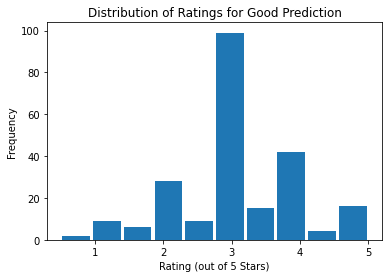
\includegraphics[width=\linewidth]{./figs/gooddist.png}
      \caption{Distribution of ratings for a well-predicted movie. The predicted and true ratings were both 3.0 stars.}
   \end{subfigure}
   \hfill
   \begin{subfigure}[b]{\columnwidth}
      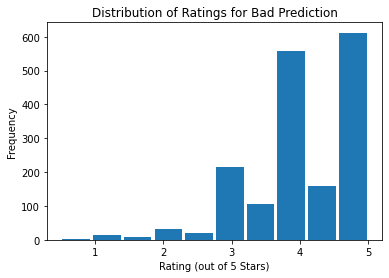
\includegraphics[width=\linewidth]{./figs/baddist.png}
      \caption{Distribution of ratings for a badly-predicted movie. The predicted and true ratings were 4.5 and 0.5 stars respectively, while the most popular ratings seem to have been 4.0 and 5.0 stars.}
   \end{subfigure}
   \caption{Rating distributions for two movies.}
\end{figure*}

\section{RESULTS}


\section{CONCLUSION}

\newpage
misc
\newpage
\bibliographystyle{IEEEtran}
\bibliography{paperbib}




\end{document}
